
%% 
%% Copyright 2007, 2008, 2009 Elsevier Ltd
%% 
%% This file is part of the 'Elsarticle Bundle'.
%% ---------------------------------------------
%% 
%% It may be distributed under the conditions of the LaTeX Project Public
%% License, either version 1.2 of this license or (at your option) any
%% later version.  The latest version of this license is in
%%    http://www.latex-project.org/lppl.txt
%% and version 1.2 or later is part of all distributions of LaTeX
%% version 1999/12/01 or later.
%% 
%% The list of all files belonging to the 'Elsarticle Bundle' is
%% given in the file `manifest.txt'.
%% 

%% Template article for Elsevier's document class `elsarticle'
%% with numbered style bibliographic references
%% SP 2008/03/01

\documentclass[preprint,12pt]{elsarticle}
%\documentclass[final,1p,times]{elsarticle}
\usepackage{lineno,hyperref}
\modulolinenumbers[5]

%\usepackage[notref]{showkeys}

%% Use the option review to obtain double line spacing
%% \documentclass[authoryear,preprint,review,12pt]{elsarticle}

%% Use the options 1p,twocolumn; 3p; 3p,twocolumn; 5p; or 5p,twocolumn
%% for a journal layout:
%% \documentclass[final,1p,times]{elsarticle}
%% \documentclass[final,1p,times,twocolumn]{elsarticle}
%% \documentclass[final,3p,times]{elsarticle}
%% \documentclass[final,3p,times,twocolumn]{elsarticle}
%% \documentclass[final,5p,times]{elsarticle}
%% \documentclass[final,5p,times,twocolumn]{elsarticle}

%% For including figures, graphicx.sty has been loaded in
%% elsarticle.cls. If you prefer to use the old commands
%% please give \usepackage{epsfig}

%% The amssymb package provides various useful mathematical symbols
\usepackage{amssymb}

\usepackage{amsmath}
\usepackage{amsfonts}
\usepackage{amssymb}
\usepackage{bm}
%% The amsthm package provides extended theorem environments
% %\usepackage{amsthm}

%% The lineno packages adds line numbers. Start line numbering with
%% \begin{linenumbers}, end it with \end{linenumbers}. Or switch it on
%% for the whole article with \linenumbers.
%% \usepackage{lineno}


\newtheorem{thm}{Theorem}
\newtheorem{lem}[thm]{Lemma}
\newdefinition{rmk}{Remark}
\newproof{pf}{Proof}
\newproof{pot}{Proof of Theorem \ref{thm2}}
\DeclareMathOperator*{\argmin}{arg\,min}

%\newtheorem{thm}{{\sc Theorem}}[section]
\newtheorem{dfn}{{\sc Definition}}[section]
\newtheorem{prp}{{\sc Proposition}}[section]
\newtheorem{lm}{{\sc Lemma}}[section]
\newtheorem{cor}{{\sc Corollary}}[section]
\newtheorem{ex}{{\sc Example}}[section]

%\journal{Reliability Engineering \& System Safety}

%% `Elsevier LaTeX' style
\bibliographystyle{elsarticle-num}
%%%%%%%%%%%%%%%%%%%%%%%

\begin{document}
\begin{frontmatter}

%\title{Elsevier \LaTeX\ template\tnoteref{mytitlenote}}
%\title{Evaluation of aging properties  by a scale-space inspection of the TTT curve\tnoteref{title1}}
\title{TTT-SiZer: A graphic tool for aging trends recognition \tnoteref{title1}}

%\tnotetext[mytitlenote]{Fully documented templates are available in the elsarticle package on \href{http://www.ctan.org/tex-archive/macros/latex/contrib/elsarticle}{CTAN}.}

%% Group authors per affiliation:
%% Group authors per affiliation:
%\author{G\'amiz, M.L.\fnref{myfootnote}}
%\fntext[myfootnote]{Corresponding author}
%\ead{mgamiz@ugr.es}
%
%\author{}
%
%\address{University of Granada}

\author[inst1]{Maria Luz G\'amiz\corref{cor1}}
\ead{mgamiz@ugr.es}

\author[inst2]{Rafael Nozal-Ca\~nadas}
%\ead{}

\author[inst1]{Roc\'io Raya-Miranda}

\cortext[cor1]{Corresponding author}


\address[inst1]{Department of Statistics and O.R., University of Granada,  Spain}
\address[inst2]{Department of Computer Science, UiT-The Arctic University of Norway , Norway}


%
%% or include affiliations in footnotes:
%\author[mymainaddress,mysecondaryaddress]{Elsevier Inc}
%\ead[url]{www.elsevier.com}
%
%\author[mysecondaryaddress]{Global Customer Service\corref{mycorrespondingauthor}}
%\cortext[mycorrespondingauthor]{Corresponding author}
%\ead{support@elsevier.com}

%\address[mymainaddress]{Dept. of Statistics and O.R.}
%\address[mysecondaryaddress]{360 Park Avenue South, New York}
%\ead{mgamiz@ugr.es}

\begin{abstract}
A new graphic tool is presented to test aging trends based on life data.  The graphical test is developed by means of scale and space inference about the Total-Time-on-Test transform and its first and second derivatives. The graphic tool TTT-SiZer is defined considering nonparametric local polynomial kernel estimators and constructing the corresponding (simultaneous as well as punctual) confidence intervals around three different curves. The finite sample properties of the method are evaluated by a simulation study and the comparison with other non-graphical tests shows that the graphical test helps localize discrepancies of empirical data concerning a given hypothesized aging property, thus allowing to solve the problem locally. 


\end{abstract}

\begin{keyword}
Total-Time-on-Test Transform \sep Kernel smoothing \sep Order statistics \sep SiZer map
\MSC[2010] 90B25 \sep  62N05
\end{keyword}

\end{frontmatter}

\linenumbers

\bigskip

\section{Introduction}
In many applications (e.g. reliability, maintainability, biometry or survival) different forms of aging are of interest giving rise to a well-known nonparametric classification of life distributions \cite{BP75}. While  ``positive aging'' describes the adverse effects of age on components or systems,  ``no aging'' means that age has no effect on residual life of an item, and  ``negative aging'' means that the item experiences certain improvement in performance with age. We are concerned with ``positive aging''.%,  however it has to be mentioned that the classification of lifetime distributions according to ``positive aging'' has a parallelism in terms of ``negative aging''. %Lay et at 

%As we know the notion of aging plays an important role in reliability and survival theory and in a technical context, 
In a technical context, aging is usually understood as a gradual decrease in performance over time, so it can be expected that the aging of a component or system increases the probability that it will fail. 

If the lifetime of a mechanism is a random variable $ X $, a natural measure of aging could be the probability of surviving above $ t + x $, assuming that the mechanism has an age of at least $ t $. This idea leads to the concept of residual life that will be formally defined later in this paper.
Another possible measure of aging is formulated in terms of the hazard function, which measures the  instantaneous propensity to the failure of a mechanism as a function of  its age. An inspection of the shape of these functions is very useful to evaluate the performance of a system in the future which is very important for making decisions in maintainability and inventory theory, for example. 
%In this sense, to identify a life distribution with a particular type of aging and then to establish a classification of families of random variables according to the concept of aging is very useful when performing  reliability and maintenance analyses of physical mechanisms.

The most commonly considered classes of life distributions can be found in \cite{BP75}, \cite{DKS86} and \cite{CW91}, among others. Although the mathematical description of aging is done under three broad categories based on hazard functions, residual life functions, and survival functions, in this paper, we will rather look at the Total-Time-on-Test curve (TTT) and we will construct a useful and novel graphic tool to characterize some important types of aging.  The TTT plot was introduced by \cite{BC75} as a tool for analysing failure data and thus some important classes of life distributions, see \cite{BK84}, are characterized in terms of the Total-Time-on-Test curve. Let us now introduce some notation and relevant definitions. Let $X$ denote a random lifetime with absolutely continuous distribution function. 

\begin{dfn} {\bf Residual life}

\noindent Let $X$ a lifetime with survival function $S$, for any fixed $t>0$ we denote $X_t$ the residual lifetime from time $t$, which represent the additional lifetime from $t$. The conditional survival function is obtained as $S_t(x)=S(t+x)/S(t)$, for all $x >0$. The mean residual time is then defined as $\mu_t= \int_0^{+\infty} \frac{S(t+x)}{S(t)}dx$. Note that $\mu_0=E[X]=\mu$.
\end{dfn}


\begin{dfn} {\bf Aging classes}

\noindent Let $X$ be a lifetime with distribution function $F$, survival function $S$ and finite mean $\mu$. We focus on classes of distributions  that are univocally described in terms of the TTT-transform.

\begin{enumerate}
\item Classification based on the failure rate
\begin{enumerate}
\item Increasing (decreasing) failure rate, $IFR$ $(DFR)$:

\noindent $X$ is {\it IFR}, if and only if, its conditional survival function is increasing. That is, for all $x>0 $ fixed, and for all $t_1 < t_2$ we have that $S_{t_1}(x) \leq S_{t_2}(x)$. This condition can be also established in terms of the hazard rate, saying that $X$ is {\it IFR} its hazard rate function given as $h(t)=f(t)/S(t)$, is increasing.

\item Upside-down Failure Rate, $UFR$:
\noindent $X$ is {\it UFR},  if and only if, its hazard function is initially increasing to a pick after declining abruptly until stabilize.

\item Bathtub shaped Failure Rate, $BFR$:
\noindent $X$ is  {\it BFR}, if and only if, its  hazard rate curve is divided into three regions: decreasing hazard rate region, constant hazard rate region, and increasing hazard rate region.
\end{enumerate}

\item Classification based on the residual life
\begin{enumerate}
\item Decreasing (increasing) mean residual life, $DMRL$:

 \noindent $X$ is {\it DMRL}, if and only if, $\mu_t$ is decreasing for all $t>0$.

\item New better than used in expectation, $NBUE$:

 \noindent $X$  is {\it NBUE} , if and only if,  $\mu_t \leq  \mu$, for all $t>0$; where $\mu_t$, defined previously, denotes the expected residual life of a mechanism with distribution $F$ and at the age $t$.

\end{enumerate}
\end{enumerate}
\end{dfn}

The following relationship can be proven: $IFR \ \Rightarrow \ DMRL \Rightarrow \ NBUE$.

The paper is organized as follows. In Section 2 we formally define the Total-Time-on-Test transform and present some relevant properties. In Section 3 we introduce local-polynomial estimators for the TTT-curve and its two first derivatives. Section 4 is devoted to SiZer map methodology. First we present the general idea and then we construct our graphic tool based on SiZer map to recognize aging trends in a lifetime by developing scale and space inferences about the TTT curve and some particular transformations of this curve. Finally we provide a graphical method for hypothesis testing. We study the good performance of the graphical test by an extensive simulation study and apply it to several real datasets in Section 5. Conclusions and future research interests are summarized in Section 6. 


\bigskip

\section{Total-Time-on-Test transform: Definition and relevant properties} \label{sec:TTT}

\subsection{Definition of TTT curve}\label{sec:TTTdef}

Total time on test plots provide a useful graphical method for tentative identification of lifetime models. This concept is very important in applications in reliability analysis. When several units are tested for studying their life lengths some of the units would fail while others may survive the test period. The sum of all observed and incomplete life lengths is the total time on test statistics. The plot of this statistic versus time is called the total-time-on-test plot. As the number of units on test tends to infinity the limit of this statistic is called the total time on test transform (TTT). This concept was introduced by \cite{BD72} and later studied by \cite{BP75}.
Model identification is based on properties of the TTT transform. 

\begin{dfn} \textbf{Total-Time-on-Test statistic} \label{ttt.def1}

\noindent Suppose $n$ items under test and successive failures are observed at $0=X_{(0)} \leq X_{(1)} \leq X_{(2)}\leq \cdots \leq X_{(n)}$, with $X_{(i)}$ the $i$-th order statistic from a lifetime random variable $X$ with absolutely continuous distribution function $F$. Then the \textit{total time on test statistic} during the interval $(0,t)$ is defined as 
\[
\tau (t) = \sum_{i=1}^r X_{(i)}+\left(n-r\right)t,
\]
provided that $X_{(r-1)}<t\leq X_{(r)}$.

\end{dfn}

For comparison purposes, usually the statistic is scaled to the interval $[0,1]$ by means of the transformation $\tau\left(X_{(r)}\right)/\tau\left(X_{(n)}\right)$, for $r=1,2,\ldots,n$.

Based on the sample order statistics we can construct the empirical distribution function, that is $F_n(t)=r/n$, for $X_{(r)} \leq t < X_{(r+1)}$, for $r=1,2,\ldots,n-1$; with $F_n(t)=0$, for $t <X_{(1)}$; and, with $F_n(t)=1$, for $t \geq X_{(n)}$. We can define the following function
\[
F^{-1}_n(p)= \inf \left\{x \geq 0:F_n(x) >p\right\},
\]
it can be checked \cite{Nair2013}, that
\[
\displaystyle{\int_0^{F^{-1}_n(\frac{r}{n})}} \left(1-F_n(t)\right)dt= \frac{\tau(X_{(r)})}{n},
\]
and also that
\[
\underset{n\rightarrow \infty}{\lim}\underset{\frac{r}{n}\rightarrow p}{\lim}\displaystyle{\int_0^{F^{-1}_n\left(\frac{r}{n}\right)}}\left(1-F_n(t)\right) dt= \displaystyle{\int_0^{F^{-1}(p)}}\left(1-F(t)\right) dt,
\]
uniformly in $p\in (0,1)$. 

\begin{dfn}\textbf{Total Time on Test transform} \label{ttt.def2} 

\noindent Let $X$ be a (non-negative) random variable with absolutely continuous cumulative distribution function $F$. The \textit{total time on test transform} of $X$ is defined as
\begin{equation} \label{ttt.curve}
\varphi(p) =\displaystyle{\int_0^{Q(p)}}\left(1-F(t)\right) dt
\end{equation}
where we denote $Q(p)= F^{-1}(p)$, for $p\in [0,1]$, the corresponding quantile function.
\end{dfn}
When $E[X] < \infty$, this expectation can be obtained as $\mu=\int_0^{Q(1)} S(t)dt$, where we denote $S(t)=1-F(t)$, the survival function. Then we define the {\textit{scaled}} TTT transform as $\varphi(p)/\mu$, for $0 \leq p \leq 1$,  which is scale invariant. We keep notation $\varphi(p)$ for the scaled TTT transform, and we assume that $\mu=1$, since it does not imply any loss of generality.


\subsection{Aging properties based on the TTT transform}\label{sec:aging}


The scaled TTT transform can be used to characterize different aging properties, see \cite{BP75} and \cite{BK84}. For $F$ the exponential distribution, it can be checked that $\varphi(p)=p$, for $0 \leq p \leq 1$. As mentioned above, based on a sample $X_1,X_2,\ldots, X_n$ one can construct the TTT plot, which will be closer to the scaled TTT curve as $n$ tends to $+\infty$. We can thus use the TTT plot as a tool for model selection, in the sense that when, for example, the TTT plot produces a cloud of points around the diagonal of the square unit, we can admit that the distribution of the underlying lifetime $F$ is exponential, that is with constant failure rate. Other failure rate shapes can be recognized from an inspection of the TTT plot. A convex TTT curve corresponds with a decreasing failure rate (DFR); a concave TTT curve corresponds with an increasing failure rate (IFR). When the TTT plot describes a trajectory first convex then concave it indicates a bathtub failure rate shape and when it is concave then convex, it indicates a unimodal failure rate shape. 

In summary, to determine the type of aging represented by $X$ we can study the shape of the TTT curve. To do it we compute the first and second derivatives of the TTT transform. Using expression \eqref{ttt.curve} can be obtained as
\begin{eqnarray*}
\varphi'(p)&=& \frac{d}{d p}\left\{\int_0^{Q(p)}S(x)dx\right\}=S\left(Q(p)\right)Q'(p)=(1-p)Q'(p); \ {\rm and}, \\
\varphi''(p)&=& -Q'(p)+(1-p)Q''(p). 
\end{eqnarray*}
where $Q'(p)=dQ(p)/dp$ and $Q''(p)=d^2Q(p)/d^2p$.

%\begin{ex}\label{expon}{Exponential distribution}
%Let $X$ be a random variable with distribution $Exp(\lambda)$.....
%\end{ex}



Let $X$ be a lifetime with distribution function $F$ and with finite mean $\mu$. From the theorems given  in \cite{Klefsjo83}, the above aging conditions can be expressed in terms of the TTT-curve as follows:
\begin{prp} {TTT-curve characterization of aging} \

\begin{enumerate}
\item $ F$ is $ IFR$, if and only if, $ \varphi'' (u) \leq  0$, for all $0 <u <1$;
\item $F$ is $DMRL$, if and only if, $ \varphi'(u) \geq  \frac{1-\varphi(u)}{1-u}$, for all $0 <u <1$;
\item $F$ is $ NBUE$, if and only if, $\varphi(u)/u \geq  1$, for all $0 <u <1$.

\end{enumerate}
 \end{prp}
%%%%%%%%%%%%%%%%%%%%%%%%%%%%%%%%%%%%%%%%%%%%%%%%%%%%%%%%%%%%%%%%%%%%%%%%%%%%%
%%%%%%%%%%%%%%%%%%%%%%%%%%%%%%%%%%%%%%%%%%%%%%%%%%%%%%%%%%%%%%%%%%%%%%%%%%%%%

%
\section{Local polynomial estimation of the TTT-transform and its first and second derivatives}\label{locpol}
%\subsection{Least-squares estimation of the Total-Time-on-Test transform with $iid$ samples} 
In this section we suggest a local-polynomial estimator for the TTT-transform directly formulated from an empirical estimation of the TTT-curve, that is, we do not need to estimate the quantiles to get an estimator of the TTT-transform.
%
\subsection{Least-squares estimation of the Total-Time-on-Test transform}

Let $X_1,X_2,\cdots,X_n$ be an independent and identically distributed random sample drawn form an absolutely continuous distribution function $F$ with density $f$. Let $X_{(1)},X_{(2)},\cdots,X_{(n)}$ denote the corresponding order statistics. Let us denote $p_i=\frac{i}{n}$ for $i= 1,2, \ldots, n$. An empirical ($naive$) estimator of the TTT-curve $\widehat{\varphi}_n$, can be defined as follows
%
\begin{equation}\label{empi}
\widehat{\varphi}_n\left(p_i\right)= \sum_{j=1}^i \left(1-\frac{j-1}{n}\right) \left(X_{(j)}-X_{(j-1)}\right),
\end{equation}
for $i=1,2,\ldots,n$, with $\widehat{\varphi}_n(0)=0$. We can observe that $\widehat{\varphi}_n(1)=\bar{X}$, the mean sample statistics. Since the properties of the curve are not affected by scale changes, we can confine the curve to be defined in the interval $[0,1]$ by first normalizing the data. That is, we work with the sample $\{X_i/\bar{X}; i=1,\ldots,n\}$. In the following, without loss of generality, we assume that $\bar{X}=1$.

Under a local-polynomial approach we consider that, for each estimation point $p_0 \in (0,1)$, the TTT-transform $\varphi(p_0)$ is locally (in a neighborhood of $p_0$) approximated by a $m$th-degree polynomial function in the sense that for all $p \in \left(p_0-h,p_0+h\right)$ we have that $\varphi(p)=\theta_0+\theta_1(p-p_0)+\theta_2(p-p_0)^2+\ldots+\theta_m(p-p_0)^m$, for an appropriate bandwidth $h$. 

The parameters of the model can be interpreted respectively as $\theta_0={\varphi}(p_0)$; ${\theta}_1={\varphi'}(p_0)$; and, in general, ${\theta}_k=\frac{\varphi^{(k)}(p_0)}{k!}$, for $k=1,2,\ldots,m$. The approximation above is valid locally if we assume certain smoothness conditions on the quantile function, in the sense of derivability. 


In particular, the three first coefficients provide the following estimates: $\widehat{\varphi}(p_0)=\widehat{\theta}$, $\widehat{\varphi}'(p_0)=\widehat{\theta}_1$, and $\widehat{\varphi}''(p_0)=2\widehat{\theta}_2$, respectively.
To this goal, we formulate the following least squares problem

\begin{eqnarray}\label{LS}
&&\left(\widehat{\theta}_0,\widehat{\theta}_1,\ldots,\widehat{\theta}_m\right)^{\intercal}= \\
\nonumber &&\underset{\left({\theta}_0,\theta_1,\ldots, {\theta}_m\right)^{\intercal}}{\arg \min} \sum_{i=1}^n\left\{\widehat{\varphi}_n(p_i)-\theta_0-\theta_1(p_i-p_0)-\ldots-\theta_m(p_i-p_0)^m\right\}^2 K_h(p_i-p_0),
\end{eqnarray}
where $K_h(\cdot)=\frac{1}{h}K(\frac{\cdot}{h})$, with $K$ a symmetric kernel function, and $h$ the bandwidth parameter that controls the size of the window around the estimation point, $p_0$, where the polynomial approximation is valid.
After differentiating in equation ($\ref{LS}$), for $m=2$ with respect to $\theta_j$ ($j=0, 1, 2$), we obtain a system of linear equations that can be written in matrix form
\begin{equation}\label{score}
\left(\begin{array}{cccc}
a_0 & a_1&\cdots &a_m \\ 
a_{1} & a_2&\cdots &a_{m+1}\\
\vdots & \vdots &\ddots &\vdots \\ 
a_m & a_{m+1}&\cdots &a_{2 m} 
\end{array}\right)
\left(\begin{array}{c}
 \theta_0 \\ 
\theta_1 \\ 
\vdots \\
\theta_m
 \end{array}\right)=
\left(\begin{array}{c} 
A_0 \\ 
A_1 \\ 
\vdots \\
A_m
 \end{array}\right);
\end{equation}
where we have denoted

\begin{equation}\label{bigA}
A_r(p_0)=\sum_{i=1}^n\widehat{\varphi}_n(p_i)(p_i-p_0)^r K_h(p_i-p_0), \ \ r=0,1,\ldots,m;
\end{equation}
and 
\begin{equation}\label{smallA}
a_l(p_0)=\sum_{i=1}^n(p_i-p_0)^l K_h(p_i-p_0), \ \ l=0,1,2,\ldots,2m.
\end{equation}

\subsubsection{Local-quadratic estimator}\label{quad}

In particular we can fit the data locally by using a 2-degree polynomial. We denote this estimator $\widehat{\varphi}_{2,h}(\cdot)$. Then, we set the least squares problem of ($\ref{LS}$) for $m=2$ and define $A_r(p_0)$ as in \eqref{bigA} for $ r=0,1,2$; and  $
a_l(p_0)$, for $ l=0, 1, 2, 3, 4$ as in \eqref{smallA}.

After differentiating in equation ($\ref{LS}$), for $m=2$ with respect to $\theta_j$ ($j=0, 1, 2$), we obtain a system of linear equations as in \eqref{score}.


We use the Cramer's rule to solve the equations and then get the estimation of the curve $\varphi$ and its derivatives at a given $p_0$, based on the quadratic fit as follows.
\subsection*{ 1. The TTT-curve:}
\begin{equation}\label{theta0}
\widehat{\varphi}_{h}(p_0)=\widehat{\theta}_0(p_0)= \sum_{i=1}^n \bar{{K}}_{0,h}\left(p_i-p_0\right) \widehat{\varphi}_n(p_i),
\end{equation}
where
\[
\bar{{K}}_{0,h}\left(p_i-p_0\right)=\frac{\left(a_1a_3-a_2^2\right)\left(p_i-p_0\right)^2+\left(a_2a_3-a_1a_4\right)\left(p_i-p_0\right)+\left(a_2a_4-a_3^2\right)}{a_0a_2a_4+2a_1a_2a_3-a_2^3-a_0a_3^2-a_1^2a_4} K_h\left(p_i-p_0\right).
\]

\subsection*{2. The first derivative:}
\begin{equation}\label{theta1}
\widehat{\varphi}'_{h}(p_0)=\widehat{\theta}_1(p_0)= \sum_{i=1}^n \bar{{K}}_{1,h}\left(p_i-p_0\right) \widehat{\varphi}_n(p_i),
\end{equation}
where explicitely we write
\[
\bar{{K}}_{1,h}\left(p_i-p_0\right)=\frac{\left(a_1a_2-a_0a_3\right)\left(p_i-p_0\right)^2+\left(a_0a_4-a_2^2\right)\left(p_i-p_0\right)+\left(a_2a_3-a_1a_4\right)}{a_0a_2a_4+2a_1a_2a_3-a_2^3-a_0a_3^2-a_1^2a_4} K_h\left(p_i-p_0\right).
\]

\subsection*{3. The second derivative: }
%In order to construct the corresponding SiZer map we are interested in the particular expression of $\widehat{\theta}_2$ (remind that $\widehat{\varphi''}(p_0)=2 \ \widehat{\theta}_2$), then we have
\begin{equation}\label{theta2}
\widehat{\varphi}''_h(p_0)=2 \widehat{\theta}_2(p_0) =2 \sum_{i=1}^n \bar{{K}}_{2,h}\left(p_i-p_0\right) \widehat{\varphi}_n(p_i)
\end{equation}
where we denote
\[
\bar{{K}}_{2,h}\left(p_i-p_0\right)=\frac{\left(a_0a_2-a_1^2\right)\left(p_i-p_0\right)^2+\left(a_1a_2-a_0a_3\right)\left(p_i-p_0\right)+\left(a_1a_3-a_2^2\right)}{a_0a_2a_4+2a_1a_2a_3-a_2^3-a_0a_3^2-a_1^2a_4} K_h\left(p_i-p_0\right).
\]
%\newpage
\bigskip

%%%%%%%%%%%%%%%%%%%%%%%%%%         LOCAL- CUBIC
\subsubsection{The local-cubic aproach}

It is convenient to increase the complexity of the model when interested in exploring shape properties through the second derivative.
 Thus we propose to carry out the local fit by using cubic polynomials. After solving the equations in \eqref{score} with $m=3$, taking  $\widehat{\varphi}_n\left(\cdot\right)$ the empirical estimator given in \eqref{empi}, we can write the estimators of $\varphi$ and its first derivatives similar to the previous section as follows.

%

%%%%%%%% TTT CURVE
\subsection*{1. The TTT-curve: }%{$\widetilde{\varphi}_h(p_0)=\widetilde{\theta}_0(p_0)$}

\noindent First, we give some notation. Let ${\bf A}$ be a square matrix of dimension $n \times n$. 

For each $i, j =1,2,\ldots, n$, denote $M_{i,j}$ corresponding $minor$, that is, the determinant of the sub-matrix obtained by deleting the $i$th row and the $j$th column of matrix ${\bf A}$. The corresponding $cofactor$ is given by  $\Delta_{ij}=(-1)^{i+j} M_{i,j}$. 

To solve the system of linear equations, we use the Cramer's rule and compute the determinants by cofactor expansions. Then we write the solution as
\begin{equation}\label{phi.cub}
\widetilde{\varphi}_h(p_0)\left(p_i-p_0\right)= \widetilde{\theta}_0(p_0)=\sum_{i=1}^n \widetilde{K}_{0,h}\left(p_i-p_0\right) \widehat{\varphi}_n\left(p_i\right)
\end{equation}
where the cubic kernel is expressed as
\begin{eqnarray*}
\widetilde{K}_{0,h}\left(p_i-p_0\right)&=& \\
&=&\frac{\Delta_{11}+\Delta_{21}\left(p_i-p_0 \right)+\Delta_{31}\left(p_i-p_0 \right)^2+\Delta_{41}\left(p_i-p_0 \right)^3}{a_0 \Delta_{11}+ a_1 \Delta_{21}+a_2 \Delta_{31}+a_3 \Delta_{41}} K_h\left(p_i-p_0\right)
\end{eqnarray*}
where the cofactors $\Delta_{ij}$, $i,j=1, 2, 3, 4$, are taken from matrix ${\bf A}$, that is,
\[
{\bf A} =\left(\begin{array}{cccc}
a_0 & a_1&a_2 &a_3 \\ 
a_{1} & a_2&a_3 &a_{4}\\
a_2 & a_3 &a_4 &a_5 \\ 
a_3 & a_4&a_5 &a_{6} 
\end{array}\right).
\]


 
%%%%First derivative:

\subsection*{2. The first derivative:} %{$\widetilde{\varphi'}_h(p_0)=\widetilde{\theta}_1(p_0)$}
\begin{equation}\label{dphi.cub}
\widetilde{\varphi}'_h(p_0)=\widetilde{\theta}_1(p_0)= \sum_{i=1}^n \widetilde{K}_{1,h}\left(p_i-p_0\right) \widehat{\varphi}_n\left(p_i\right),
\end{equation}
where
\begin{eqnarray*}
\widetilde{K}_{1,h}\left(p_i-p_0\right)&=& \\
&=&\frac{\Delta_{12}+\Delta_{22}\left(p_i-p_0 \right)+\Delta_{32}\left(p_i-p_0 \right)^2+\Delta_{42}\left(p_i-p_0 \right)^3}{a_0 \Delta_{11}+ a_1 \Delta_{21}+a_2 \Delta_{31}+a_3 \Delta_{41}}  K_h\left(p_i-p_0\right). \qquad
\end{eqnarray*}


Finally the second derivative, based on local-cubic approximation.
%%%% Second derivative:
\subsection*{3. The second derivative:}%{ $\widetilde{\varphi''}(p_0)=2\widetilde{\theta}_2(p_0)$}
\begin{equation}\label{d2phi.cub}
\widetilde{\varphi}''_h(p_0)= 2 \widetilde{\theta}_2(p_0)= \sum_{i=1}^n \widetilde{K}_{2,h}\left(p_i-p_0\right) \widehat{\varphi}_n\left(p_i\right),
\end{equation}
where 
\begin{eqnarray*}
\widetilde{K}_{2,h}\left(p_i-p_0\right)&=&\\
&=& \frac{\Delta_{13}+\Delta_{23}\left(p_i-p_0 \right)+\Delta_{33}\left(p_i-p_0 \right)^2+\Delta_{43}\left(p_i-p_0 \right)^3}{a_0 \Delta_{11}+ a_1 \Delta_{21}+a_2 \Delta_{31}+a_3 \Delta_{41}} K_h\left(p_i-p_0\right).
\end{eqnarray*}


\bigskip
%%%%%%%%%%%%%%%%%%%%%%%%%%%%%%%%%%%%%%%%%%%%%%%%%%%
%%%%%%%%%%%%%%%%%%%%%%%%%%%%%%%%%%%%%%%%%%%%%%%%%%%

\subsection{Statistical properties of the estimator}\label{stat_prop}

To derive statistical properties we write the estimators given above in terms of the corresponding $L$-estimator. That is, we re-write expressions in \eqref{theta0}-\eqref{theta2} and \eqref{phi.cub}-\eqref{d2phi.cub} each as a linear combination of the order statistics $X_{(1)} \leq X_{(2)} \leq \cdots \leq X_{(n)}$. Then we will use the results in \cite{HE2000} to obtain exact analytic expression for the bootstrap moments, in particular we will need the mean, and variance. 
We give the details for the local-quadratic case, the results for the local-cubic estimator can be derived directly.

\subsubsection{The local-quadratic estimator}

We start from the empirical estimator $\widehat{\varphi}_n$ detailed in ($\ref{empi}$), which can be expressed as
\[
\widehat{\varphi}_n(p_i)=\sum_{j=1}^i\omega_{i,j} X_{(j)},
\] 
where the weights $\omega_{i,j}$, are given by 
\[
\omega_{i,j}=\left\{\begin{array}{cll}
\frac{1}{n}, & \hspace{0.3cm}& j= 1,2, \ldots, i-1 \\
\frac{n-(i-1)}{n},& \hspace{0.3cm}& j= i \\
\end{array}\right.
\]
We can arrange these weights in matrix notation
\[
{\bf W} =\left(
\begin{array}{cccccc}
1 & 0 &0 &0& \cdots &0 \\
\frac{1}{n} & \frac{n-1}{n}&0&0&\cdots& 0 \\
\frac{1}{n} & \frac{1}{n}&\frac{n-2}{n}&0&\cdots& 0 \\
\frac{1}{n} & \frac{1}{n}&\frac{1}{n}&\frac{n-3}{n}&\cdots& 0 \\
\vdots&\vdots&\vdots&\vdots&\vdots&\vdots \\
\frac{1}{n} & \frac{1}{n}&\frac{1}{n}&\cdots&\frac{1}{n}& \frac{1}{n} \\
\end{array}
\right)
\]

\subsubsection*{The TTT-transform estimate}
\noindent From \eqref{theta0}, we have that
\begin{eqnarray*}
\widehat{\varphi}_h(p_0)&=&\sum_{i=1}^n \bar{K}_{0,h}(p_i-p_0)\sum_{j=1}^i\omega_{i,j}X_{(j)} \\
&=& \sum_{i=1}^n \sum_{j=1}^i \bar{K}_{0,h}(p_i-p_0)\omega_{i,j}X_{(j)} 
\end{eqnarray*}
re-ordering the terms in this expression we get
\begin{equation}\label{L-estim1}
\widehat{\varphi}_h(p_0)=  \sum_{j=1}^n \sum_{i=j}^n \bar{K}_{0,h}(p_i-p_0)\omega_{i,j}X_{(j)}. 
\end{equation}
Using matrix notation we can write the above expression \eqref{L-estim1} as 
\begin{equation}\label{L-estim2}
\widehat{\varphi}_h(p_0)=  \bar{\bf K}_{0,h}(p_0)^{\intercal} \cdot {\bf W} \cdot{\bf X}_{(\cdot)}, 
\end{equation}
where we have denoted the vector of weights 
$$\bar{\bf K}_{0,h}(p_0)=\left(\bar{K}_{0,h}(p_1-p_0), \bar{K}_{0,h}(p_2-p_0),\ldots,\bar{ K}_{0,h}(p_n-p_0)\right)^{\intercal},$$ and ${\bf X}_{(\cdot)}=\left(X_{(1)},\ldots,X_{(n)}\right)^{\intercal}$ is a vector that contains the ordered sample. 
%
%If denote $\bar{\bar{{ K}}}_{0,h,j}(p_0)=\sum_{i=j}^n \bar{K}_{0,h}(p_i-p_0)\omega_{i,j}$ we have that, for each fixed $p_0 \i (0,1)$, 
%\[
%\widehat{\varphi}_h(p_0)=  \sum_{j=1}^n \bar{\bar{{ K}}}_{0,h,j}(p_0) X_{(j)},  
%\]
\vskip0.3cm
We conclude that the expression \eqref{L-estim2} is an $L$-estimator. Let us define the following characteristics of the sample. The vector of means of the order statistics 
\begin{equation}\label{mean}
\boldsymbol{\mu}=\left({\mu}_{(1)},{\mu}_{(2)},\ldots,{\mu}_{(n)}\right)^{\intercal}, 
\end{equation}
with $\mu_{(i)}=E\left[X_{(i)}\right]$, for $i=1,2,\ldots,n$, and the covariance matrix 
\begin{equation}\label{var}
{\boldsymbol{\Sigma}}=\left(\begin{array}{cccc}
\sigma_{(1)}^2 & \sigma_{(12)} & \cdots & \sigma_{(1n)} \\
\sigma_{(12)} & \sigma_{(2)}^2 & \cdots & \sigma_{(2n)} \\
\vdots & \vdots & \ddots & \vdots \\
\sigma_{(1n)} & \sigma_{(2n)} & \cdots & \sigma_{(n)}^2
\end{array}\right)
\end{equation}
being $\sigma_{(i)}^2={\rm Var}(X_{(i)})$ and $\sigma_{(ij)}={\rm Cov} \left(X_{(i)},X_{(j)} \right)=E\left[\left(X_{(i)}-\mu_{(i)}\right)\cdot\left(X_{(j)}-\mu_{(j)} \right)\right]$, for $i, j= 1,2,\ldots,n$, $i<j$.

Then, it is easy to check that the variance of the estimator of the TTT-transform can be expressed as 

\begin{equation}\label{V.phi0}
{\rm Var} \left(\widehat{\varphi}_h(p_0)\right)= \bar{\bf K}_{0,h}(p_0)^{\intercal}\cdot {\bf W} \cdot {\boldsymbol{\Sigma}}\cdot  {\bf W}^{\intercal}\cdot \bar{\bf K}_{0,h}(p_0).
\end{equation}


\subsubsection*{The first derivative of the TTT-transform}


\noindent Similar to \eqref{V.phi0}  we can obtain the corresponding expression for the first derivative of the TTT-curve as
\begin{equation*}
\widehat{\varphi}'_h(p_0)=  \sum_{j=1}^n \sum_{i=j}^n \bar{K}_{1,h}(p_i-p_0)\omega_{i,j}X_{(j)}=\bar{\bf K}_{1,h}(p_0)^{\intercal} \cdot {\bf W} \cdot{\bf X}_{(\cdot)}, 
\end{equation*}
where we have defined the corresponding vector of weights 
$$\bar{\bf K}_{1,h}(p_0)=\left(\bar{ K}_{1,h}(p_1-p_0), \bar{ K}_{1,h}(p_2-p_0),\ldots,\bar{ K}_{1,h}(p_n-p_0)\right)^{\intercal},$$
the variance is 

\begin{equation}\label{V.phi1}
{\rm Var} \left(\widehat{\varphi}'_h(p_0)\right)= \bar{\bf K}_{1,h}(p_0)^{\intercal}\cdot {\bf W} \cdot {\boldsymbol{\Sigma}}\cdot  {\bf W}^{\intercal}\cdot \bar{\bf K}_{1,h}(p_0).
\end{equation}
%%%%%
\subsubsection*{The second derivative of the TTT-curve}
\noindent Finally, for the local-quadratic estimator of the second derivative of the TTT-curve we write
\begin{equation*}
\widehat{\varphi}''_h(p_0)= 2 \sum_{j=1}^n \sum_{i=j}^n \bar{K}_{2,h}(p_i-p_0)\omega_{i,j}X_{(j)}=2 \bar{\bf K}_{2,h}(p_0)^{\intercal} \cdot {\bf W} \cdot{\bf X}_{(\cdot)}, 
\end{equation*}
where we have denoted 
$$\bar{\bf K}_{2,h}(p_0)=\left(\bar{ K}_{2,h}(p_1-p_0), \bar{ K}_{2,h}(p_2-p_0),\ldots,\bar{ K}_{2,h}(p_n-p_0)\right)^{\intercal},$$
then,  we obtain the variance as 

\begin{equation}\label{V.phi2}
{\rm Var} \left(\widehat{\varphi}''_h(p_0)\right)=4  \bar{\bf K}_{2,h}(p_0)^{\intercal}\cdot {\bf W} \cdot {\boldsymbol{\Sigma}}\cdot  {\bf W}^{\intercal}\cdot \bar{\bf K}_{2,h}(p_0).
\end{equation}
%%%%%

\subsubsection{The local-cubic estimator}

For the local-cubic estimator, we proceed similarly.
\begin{eqnarray*}
\widetilde{\varphi}_h(p_0)&=&\sum_{i=1}^n \widetilde{K}_{0,h}(p_i-p_0)\sum_{j=1}^i\omega_{i,j}X_{(j)} \\
&=& \sum_{i=1}^n \sum_{j=1}^i \widetilde{K}_{0,h}(p_i-p_0)\omega_{i,j}X_{(j)},
\end{eqnarray*}
which is also an $L$-estimator. Let us denote 
$$\widetilde{\bf K}_{0,h}(p_0)=\left(\widetilde{ K}_{0,h}(p_1-p_0), \widetilde{ K}_{0,h}(p_2-p_0),\ldots,\widetilde{ K}_{0,h}(p_n-p_0)\right)^{\intercal},$$
 so we can write the variance of the estimator of the TTT-curve using the local-cubic approach as
\begin{equation}\label{V.phi0.cubic}
{\rm Var} \left(\widetilde{\varphi}_h(p_0)\right)= \widetilde{\bf K}_{0,h}(p_0)^{\intercal}\cdot {\bf W} \cdot {\boldsymbol{\Sigma}}\cdot  {\bf W}^{\intercal}\cdot \widetilde{\bf K}_{0,h}(p_0)
\end{equation}
for each $p_0 \in (0,1)$. Equally we can obtain the variance for the first and second derivatives of the local-cubic estimate.

\bigskip
%%%%%%%%%%%%%%%%%%%%%%%%%%%%%%
\subsection{Moments of order statistics}

In this section we use bootstrap techniques to estimate the first two moments of the order statistics. That is, we estimate the elements of vector $\boldsymbol{\mu}$, given in \eqref{mean}, as well as the covariance matrix $\boldsymbol{\Sigma}$ given in \eqref{var}. Let us denote the corresponding bootstrap estimators $\widehat{\boldsymbol{\mu}}$ and $\widehat{\boldsymbol{\Sigma}}$, respectively.  We consider on the one hand exact analytic expressions for these bootstrap mean and covariance matrix, and also we obtain the corresponding estimators based on Montecarlo resampling. 

\subsubsection{Exact analytic expressions}

Let $X_1,X_2,\ldots, X_n$ be a sample of independent random variables with a common absolutely continuous distribution $F$, and let  $X_{(1)} \leq X_{(2)}\leq \cdots X_{(n)}$ be the order statistics. 

First, we define $m$th non-centered moment of the $r$th order statistics as (see \cite{ABN08})
\begin{equation}\label{mu.r}
\mu_{(r)}^{(m)}=E\left[X_{(r)}^m\right]=\frac{n!}{(r-1)!(n-r)!}\int_0^1(Q(u))^m u^{r-1}(1-u)^{n-r}du,
\end{equation}
for $1\leq r \leq n$, and with $Q(u)=F^{-1}(u)$ the quantile function. We focus on $m=1,2$, because we are only interested in the mean and the variance, and as usual we compute $\sigma_{(r)}^2=\mu_{(r)}^{(2)}-\left(\mu_{(r)}\right)^2$.  
\vskip 0.5cm

We can replace $ Q(u)$ by $\widehat{Q}(u)$, and considering that $\widehat{Q}(u)= X_{(j)}$ for $(j-1)/n < u \leq j/n$ we obtain
\begin{equation}\label{mu.hat}
\widehat{\mu}_{(r)}^{(m)}=\sum_{j=1}^n\int_{(j-1)/n}^{j/n}(Q(u))^m f_B(u)du \ dv=\sum_{j=1}^n X_{(j)}^m\int_{(j-1)/n}^{j/n} f_B(u)du,
\end{equation}
where we denote $f_B(u)=\frac{n!}{(r-1)!(n-r)!} u^{r-1}(1-u)^{n-r}$, the density function of a Beta distribution with parameters $a_1=r$ and $a_2=n-r+1$. Then we conclude that the corresponding moment can be easily computed using the incomplete beta function, that is
\begin{equation}%\label{mu.hat}
\widehat{\mu}_{(r)}^{(m)}=\sum_{j=1}^n X_{(j)}^m\left[F_B\left(\frac{j}{n};a_1=r,a_2=n-r+1\right)-F_B\left(\frac{j-1}{n};a_1=r,a_2=n-r+1\right)\right],
\end{equation}
where $F_B(x;a_1,a_2)=\frac{n!}{(r-1)!(n-r)!}\int_0^x u^{a_1-1}(1-u)^{a_2-1} du$.
\bigskip

For $1 \leq r < s \leq n$, the (1,1)-order moment can be defined as 
\begin{equation}\label{mu.rs}
\mu_{(rs)}=E\left[X_{(r)}X_{(s)}\right]= _nC_{rs} \int_0^1\int_0^{u} Q(u)Q(v) u^{r-1}(v-u)^{s-r-1}(1-u)^{n-s}dvdu;
\end{equation}
where $_nC_{rs}=\frac{n!}{(r-1)!(s-r-1)!(n-s)!}$.

The double integral in \eqref{mu.rs} can be computed as
\begin{eqnarray}\label{mu.rs.hat1}
\nonumber \widehat{\mu}_{(rs)}&=&_nC_{rs}\sum_{j=2}^n \sum_{i=1}^{j-1}\int_{(j-1)/n}^{j/n}\int_{(i-1)/n}^{i/n} \widehat{Q}(u)\widehat{Q}(v) u^{r-1}(v-u)^{s-r-1}(1-u)^{n-s}dvdu +\\
&+& \sum_{j=1}^n \int_{(j-1)/n}^{j/n}\int_{(j-1)/n}^{u} \widehat{Q}(u)\widehat{Q}(v) u^{r-1}(v-u)^{s-r-1}(1-u)^{n-s}dvdu.
\end{eqnarray}
Again we replace the quantile function that appears in the integrand by its empirical version, so we get 
\begin{eqnarray}\label{mu.rs.hat2}
\nonumber \widehat{\mu}_{(rs)}&=&\sum_{j=2}^n \sum_{i=1}^{j-1} X_{(i)}X_{(j)}\int_{(j-1)/n}^{j/n}\int_{(i-1)/n}^{i/n} {_n}C_{rs} u^{r-1}(v-u)^{s-r-1}(1-u)^{n-s} dv du +\\
 &+& \sum_{j=1}^n X_{(j)}^2\int_{(j-1)/n}^{j/n}\int_{(j-1)/n}^{u} {_n}C_{rs} u^{r-1}(v-u)^{s-r-1}(1-u)^{n-s}dvdu.
\end{eqnarray}
The function inside the integrals can be interpreted in terms  of a Dirichlet distribution of order 2, which describes the distribution of a random vector $(U,V)$ according to the  bivariate density function
\begin{equation}\label{diri}
f_D(u,v)=\frac{\Gamma(a_1+a_2+a_3)}{\Gamma(a_1)\Gamma(a_2)\Gamma(a_3)}u^{a_1-1}v^{a_2-1}(1-u-v)^{a_3-1}
\end{equation}
where $0<u,v<1$, and $0<u+v<1$, and $a_1, a_2, a_3 >0$.


%%%%%%%%%%%%%%%%%%%%%%



\subsubsection{Estimation of the moments by Monte Carlo simulation}

Let $\{X_1, X_2, \ldots  X_n\}$ denote a sample of independent lifetimes identically distributed as $X$. The aim is to estimate the mean and moments of order 2 defined in the previous section by using resampling techniques. We propose Monte Carlo simulation as explained in the following algorithm. 
\subsubsection*{Algorithm 1. Bootstrapped moments of the order statistics}
\begin{enumerate}
\item[Step 1.] Draw with replacement a total of $n$ items from the set $\{1,2, \ldots, n\}$, that is: $i_1,i_2, \ldots, i_n$.
\item[Step 2.] For each $i_j$, take the corresponding $X_{i_j}$, for $j=1,\ldots, n$. Denote $X^*_{(1)} \leq X^*_{(2)}\leq  \ldots \leq X^*_{(n)}$ the resulting bootstrap order statistics sequence.  
\item[Step 3.] Repeat Step 2 up to $M$ times. Construct the $n \times M$-dimensional matrix of the form
$${\bf X}^*=\left(\begin{array} {cccc}
                     X^1_{(1)} & X^2_{(1)}&  \ldots & X^M_{(1)} \\
                     X^1_{(2)} & X^2_{(2)}&  \ldots & X^M_{(2)} \\
										 \cdots    & \cdots   &  \ddots  & \vdots    \\
									%	 X^1_{(j)} & X^2_{(j)}&  \ldots & X^M_{(j)} \\
										 \cdots    & \cdots   &  \ddots  & \vdots    \\
										 X^1_{(n)} & X^2_{(n)}&  \ldots & X^M_{(n)} \\
              \end{array}\right)$$
\item[Step 4.] Define the vector of bootstrap means $\widehat{\boldsymbol \mu}^*$, with components 
$$\widehat{ \mu}_j^*=\frac{1}{M}\sum_{m=1}^M X_{(j)}^m,$$
 for $j=1,2, \ldots, n$; and the bootstrap covariance matrix  
$$\widehat{\boldsymbol \Sigma}=(1/M)\left({\bf X}^*-\widehat{\boldsymbol \mu}^*\right)^{\intercal}\left({\bf X}^*-\widehat{\boldsymbol \mu}^*\right).$$
\end{enumerate}

\bigskip
%%%%%%%%%%%%%%%

\section{A graphic tool for evaluating aging trends}  \label{sizer1}
%\section{Development of SiZer map for evaluating aging properties}
In this section we propose a novel method to graphically test certain aging properties of the underlying lifetime distribution given a sample of life data. The graphical test is based on scale and space inference, which we explain in the following.

\subsection{Development of SiZer methods for examining the shape of the TTT-curve}
 
``SiZer'' stands for ``significant zero crossing of the derivatives'' and was introduced by \cite{CM99} and \cite{CM02} as a powerful exploratory graphical tool for density and regression functions. This tool uses kernel smoothing to estimate the structure that underlies the data, and plays with the smoothing parameter as a scale parameter to visualize the underlying characteristics in the function under study. The characteristics that ``really are there'', that is, those that are not a mere artifact of the sample variability, are revealed through the construction of confidence intervals for the first derivative of the function.
In its most well-known version, the reasoning underlying SiZer can be summarized as follows. At a bump, there is a zero crossing of the derivative. Then, all estimated slopes with different bandwidths to its left are significantly increasing while all estimated slopes to its right are significantly decreasing. In its most well-known version SiZer relies on two plots.
On the one hand, the so-called ``family plot'', which is the representation of a family of nonparametric smoothers of the target function, indexed by the bandwidth parameter. 
On the other hand, the gradient ``SiZer map'', which displays the scale and space inference about the first derivative. For each bandwidth, which corresponds to the scale,  and each value in the support, which gives localization, a confidence interval for the first derivative is calculated and the signs are displayed on the map using a color code. 

We explain a generic black-and-white version of SiZer although frequently other representations can be found in the literature.
Considering $n_h$ scales and $n_x$ localizations, each pixel in the ($n_x \times n_h$) map is coded as white if zero is greater than the upper confidence bound, indicating significant decrease;  black  if zero is less than the lower confidence bound, indicating significant increase; dark gray  if zero is within the confidence limits (no significant increase or decrease); and gray indicating regions where the data are too sparse to infer significance. 
The structure in the data is highlighted by gray changes and a change from black to white  means a significant bump. 

Several versions and adaptations of SiZer have been proposed in the literature to account for other interesting features such as curvature. Specifically there is the so called  ``SiCon'' map which is the counterpart of SiZer to display the scale and space inference about the second derivative. Thus, SiCon map is black for negative curvature (concave), white for positive curvatuve (convex), dark gray for zero curvature, and gray indicating regions where the data are too sparse. 

In this paper we take the general idea of SiZer map and develop a new graphical tool that allows to evaluate different types of aging underlying the data by means of scale and space inference about the TTT curve and its two first derivatives. We denote the method ``TTT-SiZer'' and it will rely on four plots: the TTT-plot and three color maps.


%The family plot displays in our case the bundle of estimates of the  TTT curve  obtained through the local polynomial approach presented in Section \ref{locpol} and based on a grid of bandwidths.
The first map is called ``SiZer-${\rm 0}$'' map and is obtained by interpreting the sign of the confidence intervals constructed for a convenient transformation of the TTT curve. This map will be used later to evaluate the NBUE property.
The second map is called ``SiZer-${\rm 1}$'' map and is strictly the SiZer map describe above. That is, based on the first derivative of the target curve which is the TTT curve. This plot is just for control purposes. Recall that the TTT curve is obtained as the integral of a continuous positive function, therefore increasing. The  SiZer-1 map should accordingly reflect it. 
The third map is called ``SiZer-{\rm 2}'' map and is the  SiCon  built from the inference about second derivative of the TTT curve as it is mentioned above. We use this map to evaluate deviance from non-aging (exponentiality) in favor of strong aging properties as IFR or BFR, or their duals.

%\subsection{SiZer-$k$ map, $k=0,1,2$}
Let $g_k(p)$ denote a generic function, and SiZer-${ k}$ map the corresponding color map. We consider the following notation: $g_0(p)=\varphi(p)/p-1$; $g_1(p)=\varphi'(p)$; and  $g_2(p)=\varphi''(p)$. 

Consider a grid of bandwidths (scale) and a grid of localizations in the interval $(0,1)$  (space), which is the estimation window in our case. 

Each combination of bandwidth and localization determines one pixel of a two dimensional space which will be the support of the color map. For a given bandwidth we construct the local-polynomial estimator as explained in Section \ref{locpol}. For a significance level $\alpha \in (0,1)$ we use the computation of the variance given in Section \ref{stat_prop} to build the corresponding confidence interval, that is
 
\begin{equation}\label{ci1}
\left(\widehat{g}_{k,h}(p)-q_{1-\frac{\alpha}{2}}\sqrt{{\rm \widehat{V}}\left(\widehat{g}_{k,h}(p)\right)},\widehat{g}_{k,h}(p)+q_{1-\frac{\alpha}{2}}\sqrt{{\rm \widehat{V}}\left(\widehat{g}_{k,h}(p)\right)}\right),
\end{equation}
 with $p \in (0,1)$, and $k=0,1,2$.

We are interested in determining whether 0 is inside the interval \eqref{ci1} or on the contrary the interval is strictly positive or negative. To represent each situation we use a color code as follows. A pixel is white if the upper confidence bound is lower than 0; it is black if the lower confidence  bound is greater than 0; and, it is  dark gray if zero is within the confidence limits. We use gray to color regions with sparse data.

\subsection{Motivating example}
We show the versatility of $SiZer$ for lifetime data analysis through a simulated sample. We consider a bathtub shaped failure rate distribution. In particular we simulate a sample of size $n=500$ from an additive Weibull model discussed in \cite{XieLai96} with failure rate $r(t)=(b/a)(t/a)^{(b-1)}+(d/c)(t/c)^{(d-1)}$ for $a=1;b=5;c=d=0.5$. This model is displayed in Figure \ref{Fig:simulatedhazard}.

\begin{figure}[htb]
\begin{center}
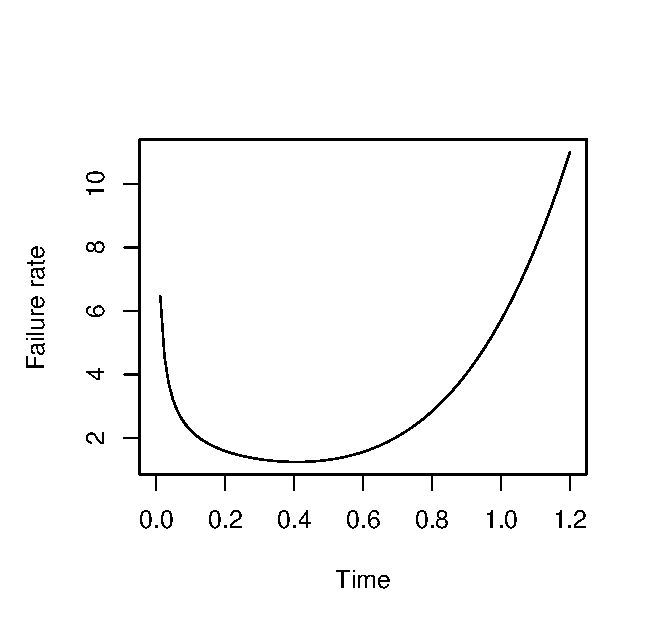
\includegraphics[height=9cm]{Fig1_motivatinghazard.eps}
\caption{Bathtub shaped failure rate.}\label{Fig:simulatedhazard}
\end{center}
\end{figure}

The results of the TTT-SiZer analysis are shown in Figure \ref{Fig:simulatedSizer}. The top-left panel shows the empirical TTT-plot for these data. The plot suggests a change of sign in convexity properties of the curve thus revealing the characteristics of the underlying  bathtub shaped failure rate. This is confirmed by the color maps which represent inferences about the TTT-curve as well as its first and second derivatives. In the top-right panel, we present the corresponding SiZer-0 map. In this case we can see a change of color in the sense white to black indicating that the TTT-transform crosses the diagonal of the unit square from below, which is in accordance with a bathtub shaped failure rate while at the same time allows to argue against the NBUE. The bottom-left panel presents the SiZer-1 map indicating positive sign of the first derivative, as expected since the TTT-curve is defined as a cumulative integral function. Finally, the bottom-right panel shows the SiZer-2 map which tells us about the second derivative. This graph picks up the true features of the underlying hazard model. 
The plot shows that the hazard rate decreases significantly at the beginning (white color up to about the point 0.5). There is then a zero-crossing  signaled by the dark gray color  (between points 0.5 and 0.7), indicating that the hazard rate is constant. The hazard rate then increases to the point 0.95, as the black color indicates. This reveals a minimum of the hazard rate around 0.5.
  

\begin{figure}[htb]
\begin{center}
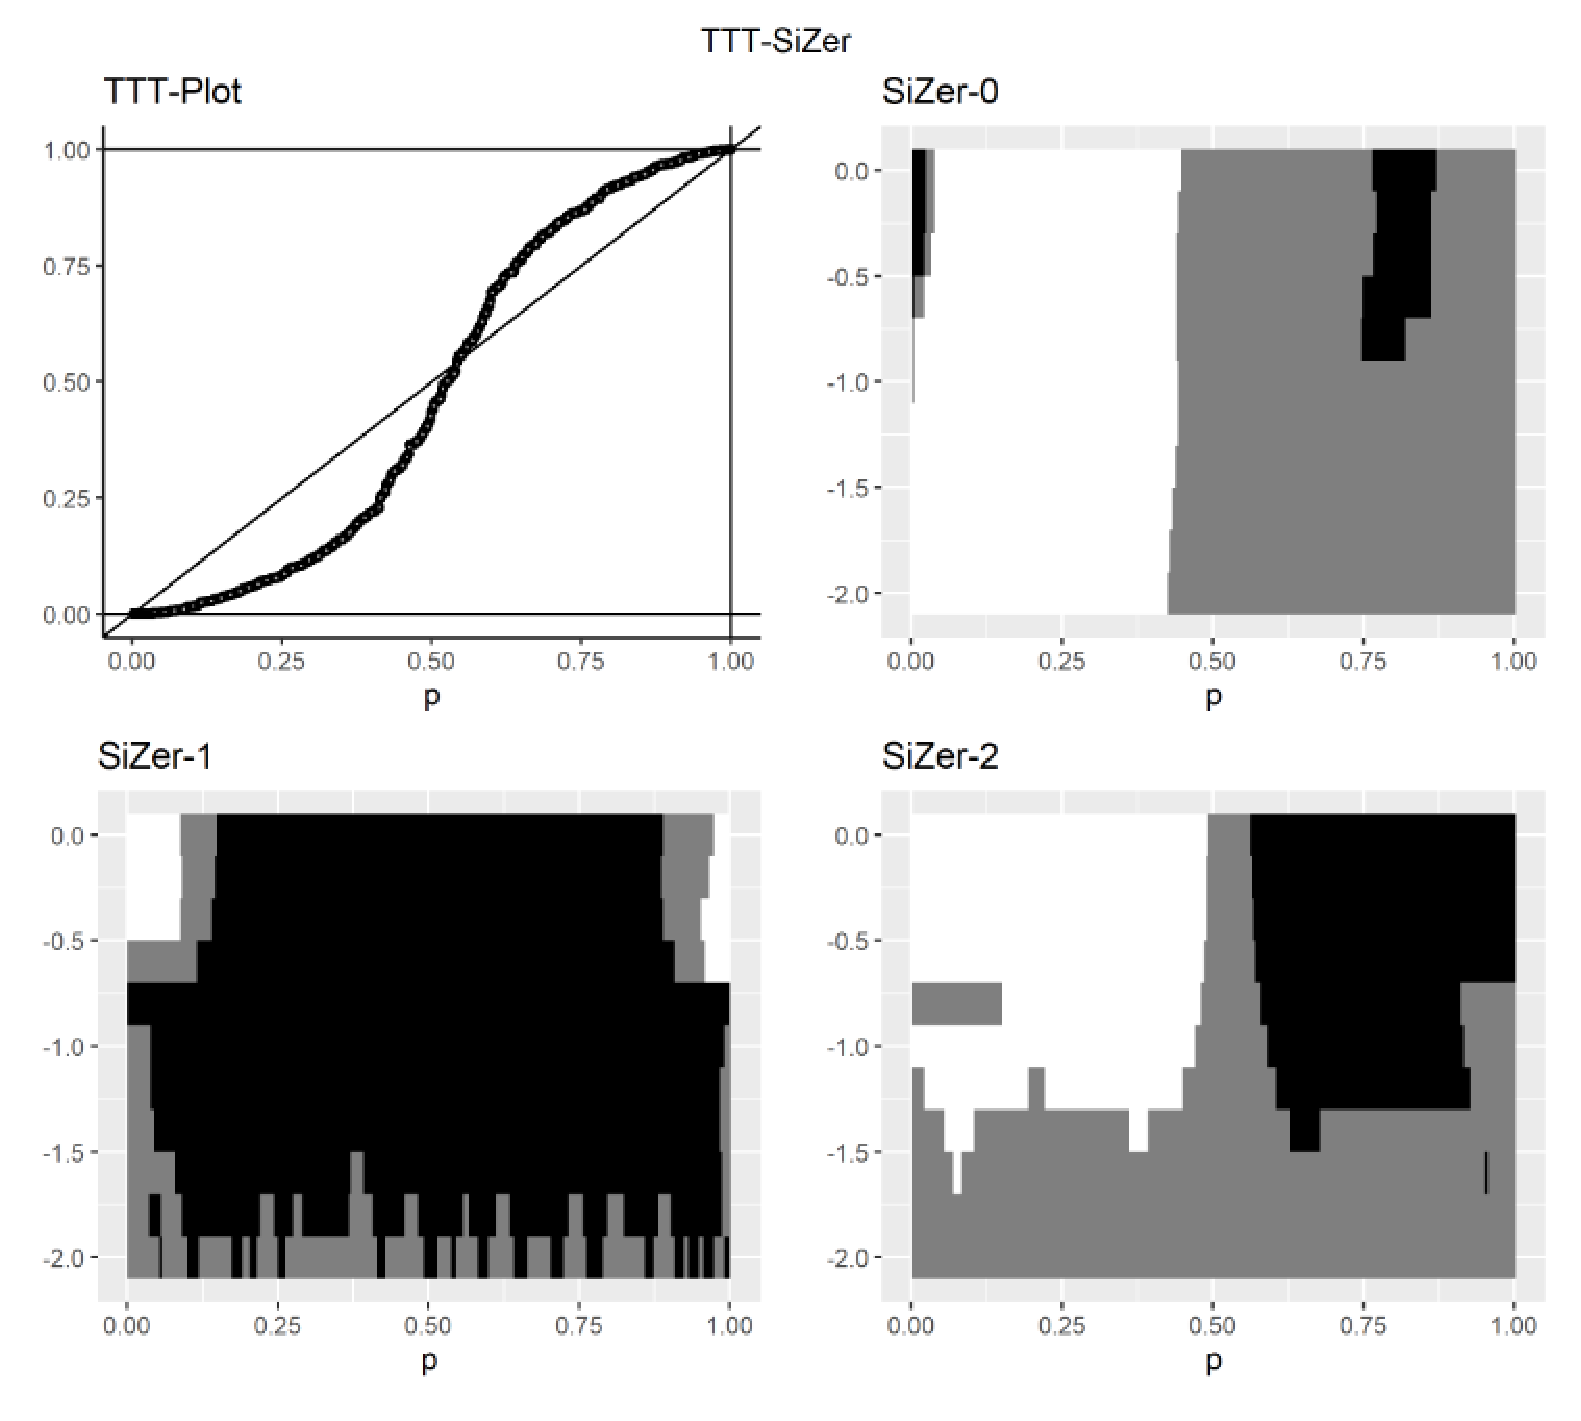
\includegraphics[height=9cm]{Fig2_motivatingSiZerCubic_log10.EPS}
\caption{TTT-Sizer for a dataset from an additive Weibull model.}\label{Fig:simulatedSizer}
\end{center}
\end{figure}

It is worth to mention at this point that, although we are using the same range of bandwidths for the three curves, it might not be the most appropriate. The second derivative implies the most complex estimation problem. More information is needed, meaning that bigger bandwidths are required. Smaller bandwidths increase variability. The resulting estimators are less efficient leading to wider confidence intervals. The wide dark gray area at the bottom of the plot in SiZer-2 shows this point.


%%%%%%%%%%%%%%%%%%%%%%%%%%%%%%%
\subsection{Some important issues in the SiZer methodology}
\begin{enumerate}
\item {\it Effective sample size} \\
\noindent The  concept of effective sample size (ESS) is considered as defined by \cite{CM99}. In this paper an estimated slope is classified to be not enough data if its ESS is less than or equal to 5, 
$$
ESS(p_0,h) = \frac{\sum_{i=1}^n K_h(p_i-p_0)}{K_h(0)}
$$
%\item {\it Kernel function}
\item {\it Quantile functions} \\
\noindent Candidates for calculation of the quantile $q$ include:
\begin{itemize}
	\item Pointwise Gaussian quantiles: $q_1(h) = q_1 = \Phi^{-1}[1-\alpha/2]$, with $\Phi$ the standard normal distribution function. 
	\item Approximate simultaneous over $p$ Gaussian quantiles: based on ``number of independent blocks'' \cite{HM2006}, defined as
	$$
	q_2(h) = \Phi^{-1} \left[\left(1- \frac{\alpha}{2}\right)^{1/\left\{\theta(\Delta)d\right\}}\right],
	$$
	where
	$$
	\theta(\Delta) =2 \Phi \left\{ \frac{\Delta \sqrt{3 \log(d)}}{2h}\right\}-1
	$$
	with $d$ the number of pixels in a row in the SiZer Map, $\Delta$ is the distance between two successive neighbouring locations $p_0$. In \cite{HM2006} the quantity $\theta(\Delta)$ is defined as the clustering index that measures the level of dependency between pixels. 
\end{itemize}
\end{enumerate}

\subsection{Hypothesis testing based on TTT-SiZer}

In this section we derive a graphical test based on TTT-SiZer  to explore aging  trends underlying in a given life dataset. The null hypothesis ($H_0$) is ``No aging'', that is the underlying lifetime is assumed to be exponentially distributed. We consider different alternative hypotheses ($H_1$)  according to the aging trend we are interested in. The kind of $H_1$ also determines the way we express the condition of ``No aging'' in $H_0$. More specifically, a classic statistical testing problem can be settled  as:

 \noindent Let $X$ be a random lifetime, we want to test the null hypothesis 
\[
{\rm H_0 :} \ X \ {\rm follows \ Exp}(\lambda) \ {\rm distribution,\ for \ some \ } \lambda >0,
\]
against general alternatives based on a sample $X_1, X_2,\ldots, X_n$ of independent copies of $X$.

In order to solve the problem using the graphical test, we first write the hypothesis terms of the TTT-transform. In this sense we mainly consider the two following problems
\begin{enumerate}

\item ``No aging'' $against$ NBUE:
\begin{eqnarray} \label{test_nbue}
\nonumber &&{\rm H_0 :} \ \varphi_X(p)= p, {\rm for \ all \ } p \in (0,1) \\
&&{\rm H_1 :} \ \varphi_X(p) >  p, {\rm for \ some \ }  p \in (0,1)
\end{eqnarray}


\item ``No aging'' $against$ IFR:
\begin{eqnarray} \label{test_ifr}
\nonumber &&{\rm H_0 :} \ \varphi_X''(p)= 0, {\rm for \ all \ } p \in (0,1) \\
&&{\rm H_1 :} \ \varphi_X''(p) < 0, {\rm for \ some \ }  p \in (0,1)
\end{eqnarray}

\end{enumerate}



We create a graphic tool composed of  four plots: the TTT-plot and the three SiZer maps which are described below.

\begin{itemize}
\item SiZer-0:
\noindent The first map is based on the sign of the following transformation of the  TTT curve: $g_0(p)=\varphi(p) - p$.
Then, we consider the corresponding $(1-\alpha)100\%$ confidence interval for $g_0(p)$, that is 

\[
\left[\widehat{\varphi}_h(p)-q_{1-\frac{\alpha}{2}}\sqrt{\widehat{V}\left(\widehat{\varphi}_h(p)\right)}-p, \ \widehat{\varphi}_h(p)+q_{1-\frac{\alpha}{2}}\sqrt{\widehat{V}\left(\widehat{\varphi}_h(p)\right) }- p \right],
\]
\noindent for $0\leq p \leq 1$.


\item SiZer-1:
\noindent The second map examines the sign of the first derivative, then we define $g_1(p)=\phi'(p)$. This map is built just for checking purposes. Since the TTT-transform is defined as the integral of a positive continuous function, it should be an increasing function, and so it should be displayed in the SiZer-1 map. %The color code for this case is:...

\item SiZer-2:
\noindent In this case we examine the sign of the second derivative of the TTT-transform. Then we have to compute confidence intervals for $g_2(p)=\varphi''(p)$. For $0\leq p \leq 1$,
\begin{equation}\label{ci_d2phi}
\left[\widehat{\varphi}''_h(p)-q_{1-\frac{\alpha}{2}}\sqrt{\widehat{V}\left(\widehat{\varphi}''_h(p)\right)}, \ \widehat{\varphi}''_h(p)+q_{1-\frac{\alpha}{2}}\sqrt{\widehat{V}\left(\widehat{\varphi}''_h(p)\right)}\right].
\end{equation}

\end{itemize}
In all cases $q$ is a proper quantile. The corresponding function $g_k(p)$, for $k =0,1,2$ is significantly positive (negative) when both confidence limits are above (below) 0, and it is not significant when 0 belongs to the confidence interval.

The general procedure consists of rewriting the hypotheses in SiZer language. To explain it we focus on \eqref{test_ifr}. The null hypothesis is equivalent to assert that the  SiZer-$2$ map underlying to the true distribution is completely dark gray. We will call this one the $true$ SiZer-2 map. We will decide to reject the null hypothesis in case that the $empirical$ SiZer-2, which is the one based on the data  displays a percentage of non-dark gray pixels above a pre-specified level. As usual we will refer to this level the type I error probability, and denote it as $\alpha$. This value is commonly taken as $\alpha=0.05$. 

We summarize the steps of our proposal in the following algorithms. 

\subsection*{Algorithm 2. Testing exponentiality $against$ hazard-trend changes} 
Define the $true$ TTT-SiZer map according to an Exponential distribution. Under this null hypothesis, SiZer-2 is completely dark gray. 
\begin{enumerate}
\item[Step 1.] Compute the sample mean $\bar{X}$ and define $\bar{X}_i=X_i/\bar{X}$, for $ i=1,2,\ldots,n$.

\item[Step 2.] Construct the $empirical$ SiZer-$2$ map as explained in Section \ref{sizer1} based on  $\{\bar{\bf X}_i; i=1, 2,\ldots, n \}$.
\item[Step 3.] Compare pixel by pixel the $empirical$ SiZer-$2$ map with the corresponding $true$ SiZer-$2$ map and count the total number of pixels where the color in the generated $empirical$ map is not the same as in the $true$ map. Define the test statistic $T_2$, as the percentage of non-dark gray pixels in the empirical map, the reported value is $T_2^0$.

\item[Step 4.] Use bootstrap methods to approximate the distribution of statistic $T_2$ under $H_0$: Draw $M$ samples of size $n$ from the $Exp(1)$ distribution. Construct the corresponding Sizer-$2$ maps and count for each the number of non-dark gray pixels, then we have a bootstrap sample of $T_2$, labelled $T^{*}_2$.

\item[Step 5.] Define the $p$-value as $p_{2,boot}=(1/M)\sum_{m=1}^M I\left\{T^{*,m}_2 > T_2^0\right\}$, with $I\{\cdot\}$ an indicator function.
\end{enumerate}
Reject the null hypothesis at a significance level of $\alpha \in [0,1]$ when $p_{2,boot} < \alpha$. %Note that we do not consider areas in the map where sparsity of data does not allow for estimation. 


%%%%%%%%%%%%%%%%%%%%%%%%%%%%%%%%%%%%%  EXAMPLES

\subsection*{Example 1. Aarset dataset, \cite{A1987}}
To demonstrate our testing method, we apply it to the dataset consisting of $n=50$ failure times of electrical devices, see for example \cite{A1987}. The results provided by classical tests are given in Table \ref{exp.test}, columns 2-3.
As suggested by the TTT-plot we want in this case to test exponentiality against BFR alternatives. The results of the TTT-SiZer method have been implemented for the local-cubic estimator and are presented in Figure \ref{Fig:aarset}. 
\begin{figure}[h]
\begin{center}
\includegraphics[height= 9cm]{Fig3_aarsetCubicPuntual_log10.EPS}
\caption{TTT-Sizer for Example 1: Electric devices failure times.}\label{Fig:aarset}
\end{center}
\end{figure}

Moreover, we have implemented Algorithm 2 for this data case. We have simulated $M=1000$ samples of size $n=50$ according to $H_0$. We have obtained $p_{2,boot}=0.044$, which leads to decision of rejecting Exponentiality, as also is suggested by the majority of testing procedures reported in Table \ref{exp.test}. Looking at the whole group of plots in Figure \ref{Fig:aarset} we can get more information than the only provided by the p-value. As already mentioned, the TTT-plot suggests the BFR condition for the underlying lifetime. This idea is confirmed by looking at both SiZer-0. This graph displays a change of sign from white to black for all bandwidths which means that the data are not in accordance with the NBUE condition. On the other hand, looking at the plot presented on SiZer-2, there is an evident change from white to black meaning a clear change of trend of the hazard rate from decreasing to increasing. So, we can conclude that the data comes from a BFR lifetime distribution. 

\subsection*{Example 2. Survival days of chronic granulocytic leukemia, \cite{BS69}}
We apply the method to the dataset consisting of survival times, in days from diagnosis, of 43 patients suffering from chronic granulocytic leukemia.%, the data can be found in \cite{KA2014}.
We consider this case to highlight the usefulness of our graphical method against other classical non-graphical tests where the decision relies on the value of an statistic and the corresponding p-value. 
Although we can also summarize our testing information in the value of a statistic as explained in Algorithm 2, the true relevance of our procedure is that we can locate areas where the null hypothesis is not supported by the data instead of only rely our decision on a single value or p-value. 

Classical tests lead to the decision of not rejecting exponentiality for this data case (see Table \ref{exp.test}, columns 4-5). Moreover, Algorithm 2 has been implemented for the local-quadratic estimator. The test statistic reported a value of $T_2^0=0.091$ with a $p_{2,boot}=0.068$. This also implies not rejecting $H_0$. However, one should be cautious with this decision since  we can appreciate a significant non-dark gray area on the left side of panel SiZer-2 that suggests an area of the interval $[0,1]$ where TTT-curve is strictly negative convex, as can be seen from Figure \ref{Fig:granu}.



\begin{table}
\centering
\caption{Some Exponentiality tests implemented in package $exptest$ \cite{NPY15} of program R.}
\begin{tabular}{|l|c|c|c|c|} \hline
&\multicolumn{2}{|c|}  {{\it Example  1. Reliability data}}  & \multicolumn{2}{|c|}{{\it Example  2. Survival time data}}\\ \hline
{\bf Test  }\cite{Ascher90} & Test Statistic & $p$-{ value} &Test Statistic &$p$-{ value} \\ \hline
Cox and Oakes        & $-3.388$ & 0.709 & $ 12.171$ & 0.148 \\ \hline
Cramer-von Mises    & $ 0.519$ &  1 & $0.149$ &  1 \\ \hline
Deshpande            & $0.708$   &  0.528 & $0.729$   &  0.127 \\ \hline 
Gini-statistic      & $ 0.411$   &  {\bf 0.031} & $0.426$   &  0.097 \\ \hline  
Gnedenko $F$-test  &  $2.236$     & {\bf 0.005 }&  $1.316$     &  0.373 \\ \hline 
Hollander- Proschan  &$0.209 $ & {\bf 0.007} &$0.225 $ & 0.125   \\ \hline 
Kochar            &  $ 3.509$ & {\bf 0.0004 } &  $2.327$ & {\bf 0.019 } \\ \hline 
Kolmogorov-Smirnov & $0.191$ & {\bf 0.005}& $ 0.162$ & {0.054}  \\ \hline 
Lorenz test        & $0.177 $& 0.870 & $ 0.191$    & 0.804\\ \hline 
Shapiro-Wilk   & $ 0.040$ & 0.996 &  $ 0.0415$ & 0.982 \\ \hline  
\end{tabular}
\label{exp.test}
\end{table}

\begin{figure}[htb]
\begin{center}
\includegraphics[height= 9cm]{Fig4_granulocyticQuadraticPuntual_01.EPS}
\caption{TTT-Sizer for Example 2: Survival days of chronic granulocytic leukemia.}\label{Fig:granu}
\end{center}
\end{figure}
%

\subsection*{Algorithm 3. Testing exponentiality $against$ NBUE alternatives} 
Define the $true$ TTT-SiZer map according to an Exponential distribution. Under this null hypothesis, SiZer-0 is completely dark gray. 
\begin{enumerate}
\item[Step 1.] Compute the sample mean $\bar{X}$ and define $\bar{X}_i=X_i/\bar{X}$, for $ i=1,2,\ldots,n$.
\item[Step 2.] Construct the  $empirical$ SiZer-$0$ map as explained in Section \ref{sizer1} based on  $\{\bar{\bf X}_i; i=1, 2,\ldots, n \}$.
\item[Step 3.] Compare pixel by pixel the $empirical$ SiZer-$0$ map with the corresponding $true$ SiZer-$0$ map and count the total number of black pixels in the generated $empirical$ map, which means that the curve is strictly above the diagonal. Define the test statistic $T_0$, as the percentage of black pixels in the empirical map, the reported value is $T_0^0$.

\item[Step 4.] Use bootstrap methods to approximate the distribution of the statistic $T_0$ under $H_0$: Draw $M$ samples from the $Exp(1)$ distribution. Construct the corresponding Sizer-$0$ maps and count for each the number of black pixels, then we have a bootstrap sample of $T_0$, labelled $T^*_0$.

\item[Step 5.] Define the $p$-value as $p_{0,boot}=(1/M)\sum_{m=1}^M I\left\{T^{*,m}_0 > T_0^0\right\}$.
\end{enumerate}
Reject the null hypothesis at a significance level $\alpha \in [0,1]$ when $p_{0,boot} < \alpha$. %Note that we do not consider areas in the map where sparsity of data does not allow for estimation. 

To illustrate this method we consider the following example. 
\subsection*{Example 3. Failure times of rear brakes, \cite{BC75}}
The third dataset represents failure times for right rear brakes on D9G-66A Caterpillar tractors \cite{BC75}. The null hypothesis of Exponential distribution is clearly rejected by classical test, and the TTT-plot also points to this decision. We have carried out our graphical test using the local-cubic estimator and paying attention to the alternative hypothesis $H_1$: ``NBUE but not Exponential distribution''. In this case the plot presented in SiZer-0 shows that data are in accordance with $H_1$. Moreover Algorithm 3 has provided a value for the statistics $T_0^0=0.663$ with a value $p_{0,boot}=0.000$, which suggests clear evidence in that sense. 

\begin{figure}[htb]
\begin{center}
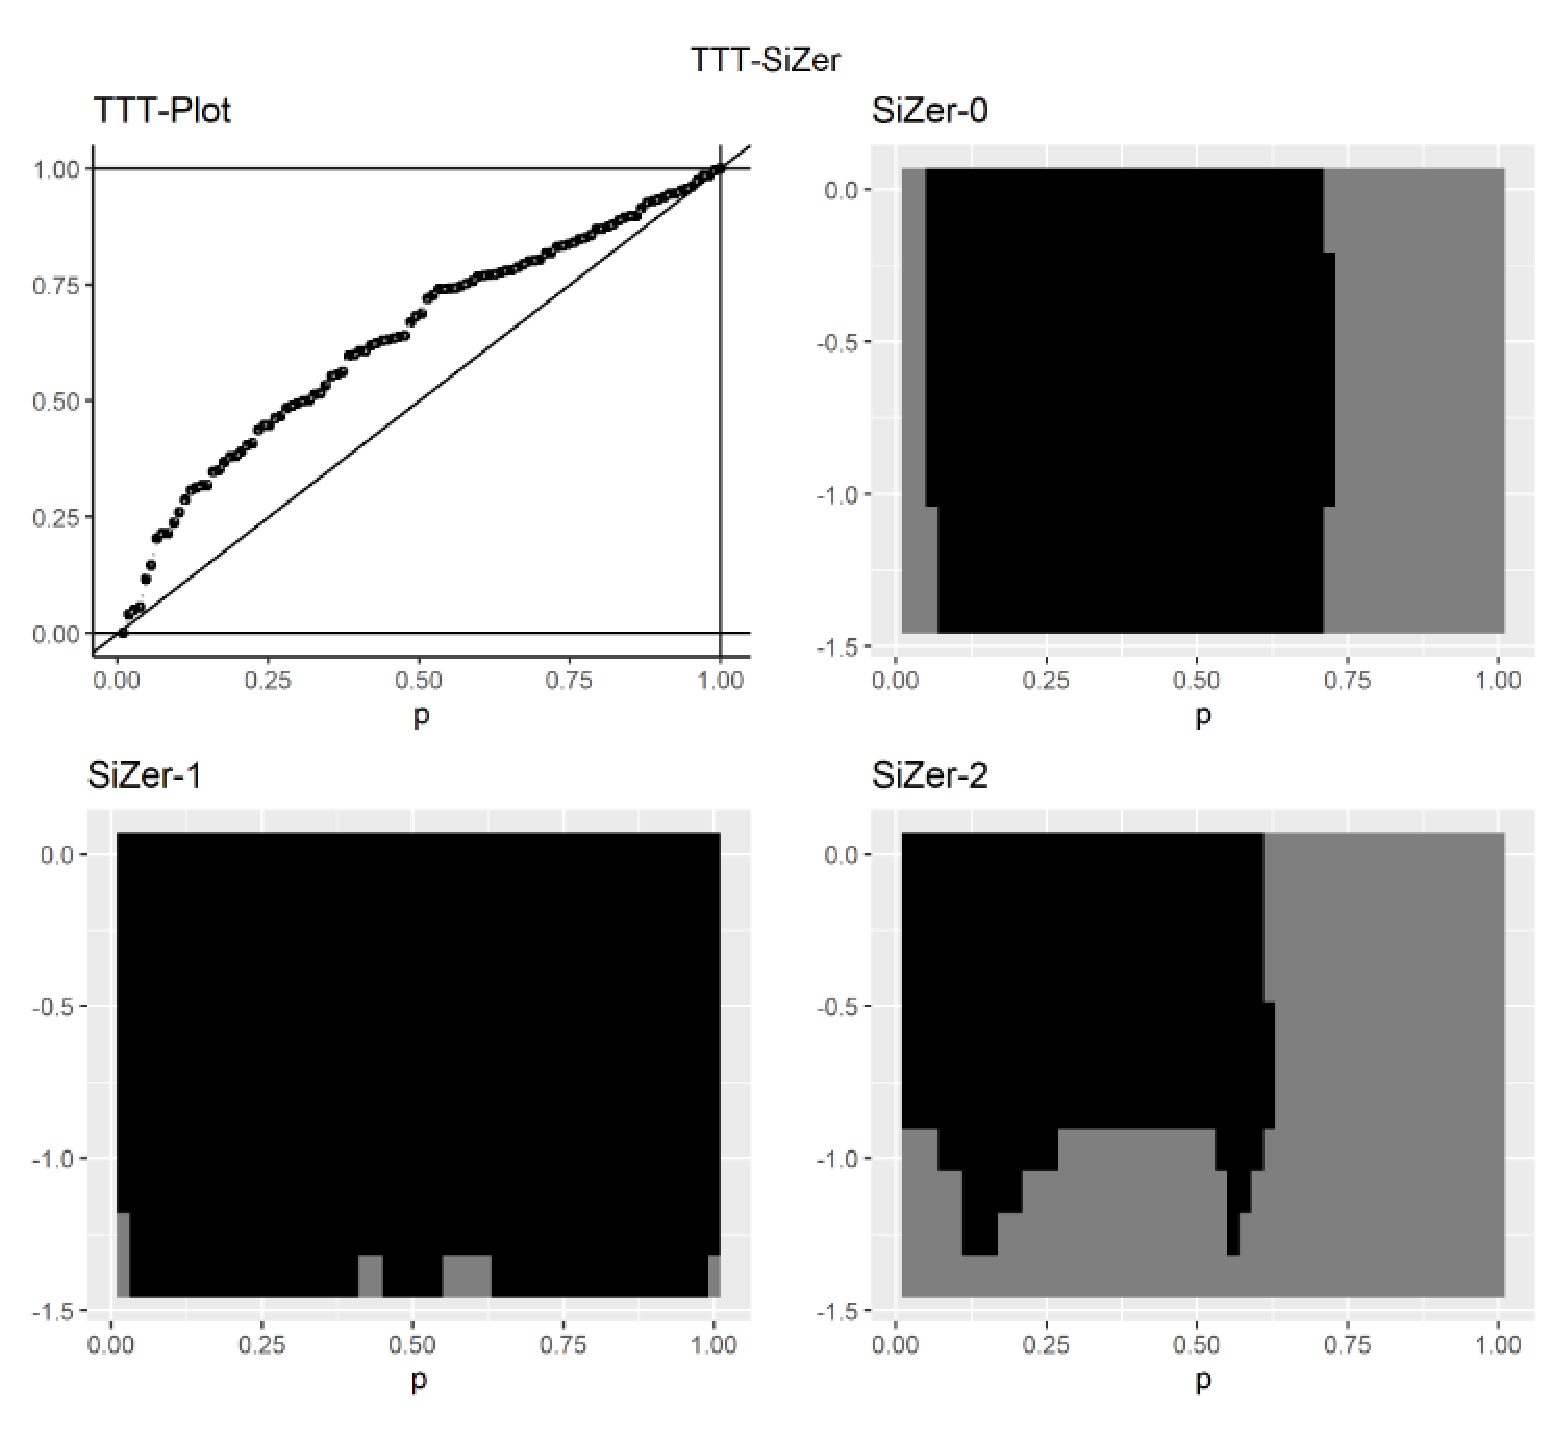
\includegraphics[height= 9cm]{Fig5_brakes_log10.EPS}
\caption{TTT-Sizer for Example 3: Failure times dataset of a brake-system.}\label{Fig:brakes}
\end{center}
\end{figure}
%

\bigskip
%%%%%%%%%%%%
\section{Simulations}\label{sec:sim}
In this section, we evaluate the performance of the graphical test. We derive the type I error of the test and the empirical power under different alternatives.% and compare with alternative non-graphical tests.

\subsection{Type I error}
The type I error occurs when the graphical test rejects the true model under the null hypothesis. To evaluate the type I error of the graphical TTT-test, we simulate samples of size $n = 100, 500$, and $1000$, from an Exponential distribution with mean 1.

The TTT-transform and its second derivative are estimated using the local polynomial estimators defined in Section \ref{locpol}, with gaussian kernel. We apply the  TTT-SiZer method to visualize the inference about the second derivative in a two dimensional space with $np \times nh$ pixels.  
The algorithm consists of simulating a sample of size $n$ from the true model, then we calculate the local-polynomial estimate and apply the TTT-SiZer method to compare the corresponding SiZer-2 map with the true one.

To measure the probability of committing this error we follow \cite{RMP07}. We focus on the null hypothesis of $No \ aging$ and consider as alternative $H_1$: ``Aging \ trend''.
As remarked above, under the null hypothesis that the TTT-curve is the diagonal of the unit square, the SiZer-2 map  should have only dark gray pixels. We consider this map as the true one. We repeat the experiment $M=1000$ times.  For all the $M$ simulated samples, we construct the corresponding maps and compare them with the true map, pixel by pixel. For each sample, we count the total number of pixels where the color in the generated map is the same as in the true map. The proportion of type I errors for each sample is this count divided by the total number of pixels in the map. We obtain $M$ proportions of type I errors (one for each simulated sample) for each sample size. Table \ref{Tab:errorI} presents the results of the experiment. 


Table \ref{Tab:errorI}  shows that the mean of the proportions of type  I error is under 5\% for all sample sizes, as well as the median. 

\begin{table}[htb]
\centering
\caption{Summary of the type I errors calculated from $M=1000$ simulated samples, for the null hypothesis of $ H_0$: No aging.}
{\begin{tabular}{r|ccccccc}
 %$SiZer-0$      &   Sample size & Mean &   Min.    & Median & $P_{75}$ & $P_{95}$& Max.  \\
%\hline
%& 100       &0.015 & 0.000  &  0.000 &0.000  & 0.091& 0.497\\
%& 500     & 0.012&0.000  &0.000  &0.004  &0.069  &0.512\\
%& 1000      &0.011 &0.000  &0.000  &0.002  & 0.059 &0.616\\ \hline \hline
   Sample size & Mean &   Min.     & Median & $P_{75}$ & $P_{95}$& Max. \\ \hline
      50     & 0.036 & 0.000 & 0.000 & 0.017 &0.177 &0.696 \\
     100     & 0.033 & 0.000 & 0.001 & 0.026 &0.176 &0.516 \\
     500     & 0.028 & 0.000 & 0.008 & 0.027 &0.120 &0.344\\
     1000    & 0.035 & 0.000 & 0.013 & 0.034 &0.156 &0.358\\ \hline
\end{tabular}}
\label{Tab:errorI}
\end{table}

\subsection{Empirical power}

In hypothesis testing the power is defined as the probability of rejecting the null hypothesis when it is false. The probability of accepting the null hypothesis when false is called type II error. To evaluate the power of the graphical TTT-test, we consider three  different aging models and  simulate samples of size $n = 100, 500$, and $1000$, for each model as in the previous section.  In particular we consider:
\begin{itemize}
\item IFR model: $X_1$ with Gamma distribution with shape parameter $sh=5$ and mean $\mu=1$;
\item BFR model: $X_2= \min\{W_1, W_2, W_3\}$, where $W_j$ has Weibull distribution with scale $sc=2.5$, and respectively, shape parameters given by $sh_1=3$, $sh_2=2$, and, $sh_3=0.5$;
\item UFR model: $X_3$ with log-Normal distribution with parameters $E[ \log (X_3)]=-0.5$, and $Var(\log(X_3))=1$.
\end{itemize}
In all cases the parameters have been chosen to have mean around 1 and avoid scale adjustments of the TTT transform. A picture of the corresponding hazards is given in Figure \ref{models}.

The TTT-transform and its first and second derivative are estimated using the local polynomial estimators defined in Section \ref{locpol}, with gaussian kernel. We apply the TTT-SiZer method to visualize the inference about the three curves considering for each case the corresponding two dimensional space with $np \times nh$ pixels, respectively.  

\begin{figure}[h]\centering
        \includegraphics[height=5cm]{Fig6_1_IFRmodel.eps}
				\includegraphics[height=5cm]{Fig6_2_BFRmodel.eps}
				\includegraphics[height=5cm]{Fig6_3_UFRmodel.eps}
\caption{{Hazard functions for the three aging models considered}.} \label{models}
\end{figure}

The algorithm now consists of simulating a sample of size $n$ from the true model, then we calculate the local-polynomial estimate and apply the TTT-SiZer method to compare the corresponding set of maps with the true ones.
The type II error occurs when the graphical test accepts the null hypothesis under the alternative. To measure the probability of committing this error we follow again \cite{RMP07}. We focus on the three different models that represent aging trends is some way. Under the null  hypothesis, the SiZer-2 map  should have only dark gray pixels. We consider this map as the true one. We repeat the experiment $M=1000$ times.  For each of the $M$ simulated samples, we construct the corresponding maps and compare them with the true map, pixel by pixel. For each sample, we count the total number of pixels where the color in the generated map is  the same as in the true map. The proportion of type II errors for each sample is this count divided by the total number of pixels in the map. We obtain $M$ proportions of type II errors (one for each simulated sample) for each sample size. The empirical power is obtained as one minus this proportion. Table \ref{Tab:power} presents the results of the experiment.


\begin{table}[htb]
\centering
\caption{Summary of empirical power calculated from $M=1000$ simulated samples.}
{\begin{tabular}{llllllll}
  $H_1$   & Sample size &   Mean & Min. & Median   & $P_{75}$ & $P_{95}$& Max.\\
\hline
IFR model &50        & 0.746& 0.035 & 0.771 & 0.805  & 0.861 & 0.908\\
          &100       & 0.651& 0.444 & 0.654 & 0.679  & 0.711 & 0.747\\
          &500       & 0.517& 0.461 & 0.518 & 0.529  & 0.544 & 0.560\\
          &1000      & 0.557& 0.521 & 0.558 & 0.567  & 0.580 & 0.589\\ \hline
BFR model &50        & 0.184& 0.000 & 0.143 & 0.234  & 0.610 & 0.762\\
          &100       & 0.243& 0.000 & 0.221 & 0.285  & 0.528 & 0.647\\
          &500       & 0.390& 0.240 & 0.398 & 0.454  & 0.490 & 0.525\\
          &1000      &0.499 & 0.360  & 0.516 & 0.533  & 0.552 & 0.568\\ \hline
UFR model &50        &0.050 & 0.000 & 0.008 & 0.043  & 0.340 & 0.670\\
          &100       &0.093 & 0.000  & 0.089 & 0.098  & 0.456 & 0.600 \\
          &500       &0.305 & 0.006  & 0.350 & 0.403  & 0.445 & 0.495\\
          &1000      &0.430 & 0.157  & 0.448 & 0.471  & 0.490 & 0.506\\ \hline

\end{tabular}}
\label{Tab:power}
\end{table}

Note that for sample sizes $n=500, 1000$ the maps have been built taking in total $401 \times 11$ pixels, whereas for $n=100$, $51 \times 11$ pixels, and for $n=50$ we have considered $21 \times 11$ pixels in the maps, which means that the results are not fully comparable. Table \ref{Tab:power} shows the good performance of our test given that the results presented in the table imply a percentage of rejection is reasonable to high for almost all models and sample sizes. Especially when the alternative hypothesis is monotone. Only for the UFR case and small sample sizes, we get a small percentage of pixels allowing us to detect the alternative hypothesis in the data. For the rest of the models and sample sizes, the graphical test displays wide areas in the corresponding plots properly recognizing the alternative hypothesis.


\section{Concluding remarks}
This paper has aimed to present a new procedure to explore life data for discovering aging trends in the underlying life distribution. We have developed a graphic tool to test Exponentiality against alternatives that represent non-constant trends in aging.  The graphical test is developed through scale and space inference about the Total-Time-on-Test transform which is implemented by adapting the SiZer methodology to our context.
We have constructed local-polynomial estimators for the TTT-curve and its first and second derivatives. To obtain the properties of the estimators we need to estimate the moments of the order statistics and we have considered bootstrap methods for this purpose. We have constructed punctual as well as simultaneous confidence intervals around each curve and for different levels of smoothing. The graphical representation allows one to detect and confirm monotone aging trends and/or changes of tendency.
Simulations and the comparison with other non-graphical tests show that the graphical test helps localize discrepancies of empirical data concerning a given hypothesized aging property. A natural extension of the method is to consider more general scenarios where censoring and/or other filtering schemes are present in the sampling mechanism.

\begin{thebibliography}{}
% Los años al final de la referencia
%\bibitem{ABGK1993}

\bibitem{A1987} Aarset, M.V. (1987) How to identify a bathtub hazard rate. {\it IEEE Transactions on Reliability}, 36 (1), 106--108.

\bibitem{AG2020} Ahmad, A.E-B.A. and Ghazal, M.G.M, (2020) Exponentiated additive Weibull distribution. {\it Reliability Engineering and System Safety}, 193, https://doi.org/10.1016/j.ress.2019.106663.

\bibitem{ABN08} Arnold, B.C., Balakrishnan, N. and Nagaraja, H.N. (2008) \textit{A First Course in Order Statistics. Classics in Applied Mathematics}. New York: Willey. 

\bibitem{Ascher90} Ascher, S. (1990) A survey of tests for exponentiality. {\it Communications in Statistics- Theory and Methods}, 19 (5), 1811--1825.

\bibitem{BC75} Barlow, R.E. and Campo, R. (1975) Total time on test processes and applications to failure data analysis. In \textit{Reliability and Fault Tree Analysis}, Edited by: Barlow, R.E., Fussell, J. and Singpurwalla, N.D. 451--481.

\bibitem{BD72} Barlow, R. E. and Doksum, K.A. (1972) Isotonic test for convex ordering. \textit{Procedings of the 6$th$ Berkeley Symposium on Mathematical Statistics and Probability}, Vol. 1, pp. 293--323, University of California Press.

\bibitem{BP75} Barlow, R. E. and Proschan, F. (1975) \textit{Statistical theory of reliability and life testing}. Holt, Rinehart and Winston.

\bibitem{BK84} Bergman, B. and Klefsjö, B. (1984) The Total Time on Test Concept and Its Use in Reliability Theory. \textit{Operations Research}, 32 (3), \textit{Reliability and Maintainability},  596--606.

%\bibitem{BL83} Bergman and Lindqvist (1983)

 \bibitem{BS69} Bryson M.C. and Siddiqui, M.M. (1969) Some criteria for aging. \textit{Journal of the American Statistical Association},  64, 1472-–1483. 

\bibitem{CW91} Cao, J. and Wang, Y. (1991) The NBUC and NWUC classes of life distributions. \textit{Journal of Applied Probability}, 28, 473--479.

\bibitem{CM99} Chaudhuri, P. and Marron, J.S. (1999)  SiZer for Exploration of Structures in Curves. \textit{Journal of the American Statistical Association}, 94 (447),  807--823.

\bibitem{CM02} Chaudhuri, P. and Marron, J.S. (2002) Curvatuve vs. Slope Inference for Features in Nonparametric Curve Estimates. {\it Unpublished manuscript}.

\bibitem{DKS86} Deshpande, J.V., Kochar, S.C. and Singh, H. (1986) Aspects of positive ageing. \textit{Journal of Applied  Probability}, 23, 748--758.

\bibitem{HM2006} Hannig, J. and Marron, J.S. (2006) Advanced Distribution Theory for SiZer. \textit{Journal of the American Statistical Association}, 101 (474). 

\bibitem{HE2000} Hutson, A.D. and Ernst, M. (2000) The exact bootstrap mean and variance of an L-estimator. \textit{Journal of the Royal Statistic Society} B. Vol. 62, Part 1, pp. 89--94.

\bibitem{HP72}  Hollander, M. and Proshan, F. (1972) Testing whether new is better than used. {\it Annals of Mathematical Statistics},  43, 1136--1146.

%\bibitem{KA2014} Kattumannil, P.A. (2014) An exact test against decreasing mean time to failure class alternatives. {\it Technical Report RM 704, Department of Statistics and Probability, Michigan State University}.

\bibitem{Klefsjo83} Klefsjö, B. (1983) Some tests against aging based on Total Time on Test Transform. {\it Communications in Statistics - Theory and Methods} 12, (8) 907--927.


\bibitem{Kochar85} Kochar, S.C. (1985) Testing exponentiality against monotone failure rate average. {\it Communications in Statistics –- Theory and Methods}, vol. 14, pp. 381–392.

\bibitem{KL98} Kvaløy, J.T. and Lindqvist, B.H. (1998) TTT-based tests for trend in repairable systems data. {\it Reliability Engineering and System Safety}, 60 (1), 13--28.

%\bibitem{KS88} Kochar and Singh (1988) 

%\bibitem{Lay2006} Lay{\it et al.} (2006)


\bibitem{Nair2013} Nair, N.U., Sankaran, P.G. and Balakrishnan, N. (2013) {\it Quantily-based reliability analysis}. Birkhauser.

\bibitem{NPY15} Novikov, A., Pusev, R. and Yakovlev, M. (2015) Package ''exptest''.  https://CRAN.R-project.org/package=exptest.

\bibitem{RMP07} Rondonotti, V., Marron, J.S., and Park C. (2007) SiZer for time series: A new approach to the analysis of trends. {\it Electronic Journal of Statistics}, 1, 268--289.

\bibitem{XieLai96} Xie, M. and Lai, C.D. (1996) Reliability analysis using and additive Weibull model with bathtub-shaped failure rate function. {\it Reliability Engineering and System Safety}, 52 (1), 87--93.
\end{thebibliography}


\end{document}
